\documentclass{article}
\usepackage[utf8]{inputenc}
\usepackage{hyperref}
\usepackage{amsthm}
\usepackage{amsmath}
\usepackage{enumitem}
\usepackage{amssymb}
\usepackage{tikz}
\usepackage{tikz-cd}
\usetikzlibrary{positioning}
\usetikzlibrary{arrows,calc,patterns,positioning,shapes}
\usetikzlibrary{decorations.pathmorphing}
\usepackage{graphicx}
\usepackage{float}
%\usepackage{buzzproof}
\usepackage{bussproofs}
\usepackage{bussproofs-extra}
\usepackage{}

\title{PHIL 143 Hw4}
\author{Jad Damaj}
\date{February 14, 2024}

\usepackage{geometry}
\geometry{a4paper, margin=1in}

\newcommand{\bZ}{\mathbb{Z}}
\newcommand{\bR}{\mathbb{R}}
\newcommand{\bQ}{\mathbb{Q}}
\newcommand{\bF}{\mathbb{F}}
\newcommand{\bC}{\mathbb{C}}
\newcommand{\bN}{\mathbb{N}}
\newcommand{\bH}{\mathbb{H}}
\newcommand{\ex}{\exists}
\newcommand{\fa}{\forall}
\newcommand{\ve}{\varepsilon}
\newcommand{\from}{\leftarrow}
\newcommand{\ifff}{\leftrightarrow}
\newcommand{\cT}{\mathcal{T}}
\newcommand{\vn}{\varnothing}
\newcommand{\vp}{\varphi}
\newcommand{\cB}{\mathcal{B}}
\newcommand{\cC}{\mathcal{C}}
\newcommand{\cL}{\mathcal{L}}
\newcommand{\cM}{\mathcal{M}}
\newcommand{\cP}{\mathcal{P}}
\newcommand{\cN}{\mathcal{N}}

\newcommand{\im}{\text{im }}
\newcommand{\Tot}{\text{Tot}}
\newcommand{\dom}{\text{dom}}
\newcommand{\val}{\text{val}}
\newcommand{\sub}{\text{sub}}
\newcommand{\len}{\text{len}}

\newcommand{\To}{\Rightarrow}

\tikzset{
    modal/.style={>=stealth',shorten >=1pt,shorten <=1pt,auto,
                     node distance=1.5cm,semithick},
    world/.style={circle,draw, fill=gray!15, minimum size =0.6cm},
    bworld/.style={circle, draw, fill = gray!75},
    }

\theoremstyle{definition}
\newtheorem{exercise}{Exercise}

\begin{document}

\maketitle

\begin{exercise}
    Draw the filtration of each model through the given formula.  
    \begin{enumerate}[label = (\alph*)]
        \item $p \to \lozenge p$
        \[ 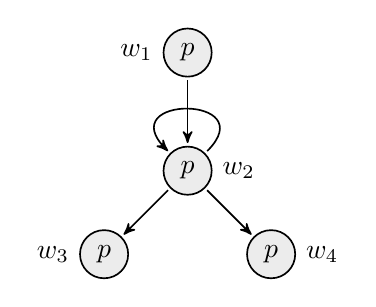
\begin{tikzpicture}[modal]
            \node[world] (w1) [label=left: {$w_1$}] {$p$};
            \node[world] (w2) [below of=w1, label=right:{$w_2$}] {$p$}; 
            \node[world] (w3) [below right of=w2, label=right:{$w_4$}] {$p$}; 
            \node[world] (w4) [below left of=w2, label=left:{$w_3$}] {$p$};

            \path[->] (w2) edge[in=135, out=45, loop, looseness=6] (w2);
            \path[->] (w1) edge[] (w2); 
            \path[->] (w2) edge[] (w3); 
            \path[->] (w2) edge[] (w4);
        \end{tikzpicture}\]
        \item $\square p \to \square \square p$
        \[ 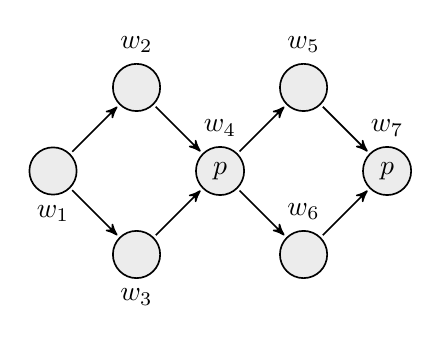
\begin{tikzpicture}[modal]
            \node[world] (w1) [label=below: {$w_1$}] {}; 
            \node[world] (w2) [above right of=w1, label=above: {$w_2$}] {};
            \node[world] (w3) [below right of=w1, label=below: {$w_3$}] {};
            \node[world] (w4) [below right of=w2, label=above: {$w_4$}] {$p$};
            \node[world] (w5) [above right of=w4, label=above: {$w_5$}] {};
            \node[world] (w6) [below right of=w4, label=above: {$w_6$}] {}; 
            \node[world] (w7) [above right of=w6, label=above: {$w_7$}] {$p$};

            \path[->] (w1) edge[] (w2);
            \path[->] (w1) edge[] (w3);
            \path[->] (w2) edge[] (w4);
            \path[->] (w3) edge[] (w4);
            \path[->] (w4) edge[] (w5);
            \path[->] (w4) edge[] (w6);
            \path[->] (w5) edge[] (w7);
            \path[->] (w6) edge[] (w7);
        \end{tikzpicture}\]
        \item $p \to \lozenge p$
        \[ 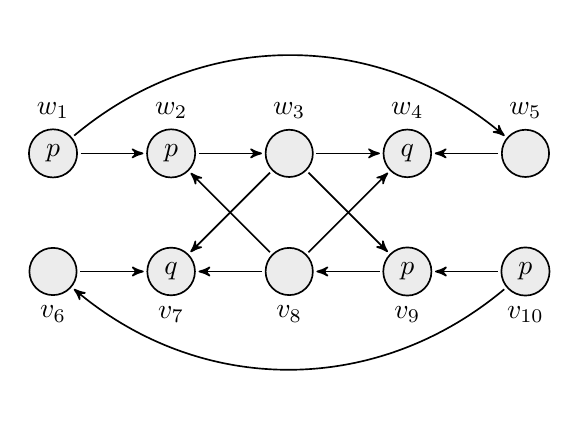
\begin{tikzpicture}[modal]
            \node[world] (w1) [label=above:{$w_1$}] {$p$}; 
            \node[world] (w2) [right of=w1, label=above: {$w_2$}] {$p$};
            \node[world] (w3) [right of=w2, label=above: {$w_3$}, minimum size=0.6cm] {}; 
            \node[world] (w4) [right of=w3, label=above: {$w_4$}] {$q$};
            \node[world] (w5) [right of=w4, label=above: {$w_5$}] {};

            \node[world] (v1) [below of=w1, label=below: {$v_6$}] {};
            \node[world] (v2) [below of=w2, label=below: {$v_7$}] {$q$};
            \node[world] (v3) [below of=w3, label=below: {$v_8$}] {};
            \node[world] (v4) [below of=w4, label=below: {$v_9$}] {$p$};
            \node[world] (v5) [below of=w5, label=below: {$v_{10}$}] {$p$};

            \path[->] (w1) edge[] (w2); 
            \path[->] (w2) edge[] (w3);
            \path[->] (w3) edge[] (w4); 
            \path[->] (w5) edge[] (w4);

            \path[->] (v1) edge[] (v2); 
            \path[->] (v3) edge[] (v2);
            \path[->] (v4) edge[] (v3); 
            \path[->] (v5) edge[] (v4);

            \path[->] (w3) edge[] (v2); 
            \path[->] (w3) edge[] (v4);
            \path[->] (v3) edge[] (w2); 
            \path[->] (v3) edge[] (w4);

            \path[->] (w1) edge[bend left=40] (w5);
            \path[->] (v5) edge[bend left=40] (v1);
        \end{tikzpicture} \]
    \end{enumerate}
\end{exercise}

\begin{proof} \mbox{}
    \begin{enumerate}[label = (\alph*)]
        \item \mbox{} 
        \[ 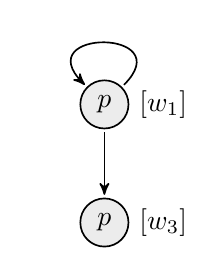
\begin{tikzpicture}[modal]
            \node[world] (w1) [label=right: {$[w_1]$}] {$p$}; 
            \node[world] (w3) [below of=w1, label=right: {$[w_3]$}] {$p$};

            \path[->] (w1) edge[in=135, out=45, loop, looseness=6] (w1);
            \path[->] (w1) edge[] (w3);
        \end{tikzpicture}\]
        \item \mbox{} 
        \[ 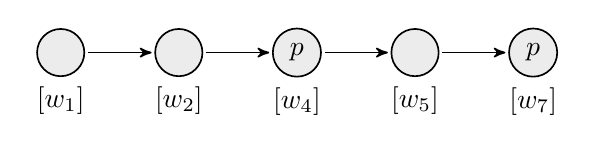
\begin{tikzpicture}[modal]
            \node[world] (w1) [label=below: {$[w_1]$}] {}; 
            \node[world] (w2) [right of=w1, label=below: {$[w_2]$}] {}; 
            \node[world] (w3) [right of=w2, label=below: {$[w_4]$}] {$p$}; 
            \node[world] (w4) [right of=w3, label=below: {$[w_5]$}] {}; 
            \node[world] (w5) [right of=w4, label=below: {$[w_7]$}] {$p$}; 

            \path[->] (w1) edge[] (w2); 
            \path[->] (w2) edge[] (w3); 
            \path[->] (w3) edge[] (w4); 
            \path[->] (w4) edge[] (w5);
        \end{tikzpicture}\]
        \item \mbox{} 
        \[ 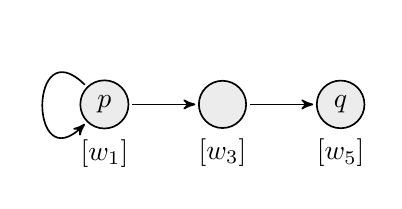
\begin{tikzpicture}[modal]
            \node[world] (w1) [label = below: {$[w_1]$}] {$p$}; 
            \node[world] (w3) [right of=w1, label = below: {$[w_3]$}] {}; 
            \node[world] (w5) [right of=w3, label = below: {$[w_5]$}] {$q$};

            
            \path[->] (w1) edge[] (w3); 
            \path[->] (w3) edge[] (w5); 
            \path[->] (w1) edge[in=225, out=135, loop, looseness=6] (w1);
        \end{tikzpicture}\]
    \end{enumerate}
\end{proof}

\begin{exercise} \mbox{}
    \begin{enumerate}[label = (\alph*)]
        \item Prove that if a formula $\vp$ contains $n$ connectives, then $|\sub(\vp)| \le 2n+1$. 
        \item Show that the bound is sharp. That is, for any $n$, give an example of formula with $n$ connectives and exactly $2n+1$ subformulas. 
    \end{enumerate}
\end{exercise}

\begin{proof} \mbox{} 
    \begin{enumerate}[label = (\alph*)]
        \item We show this by induction on the complexity of the formula. \\ 
        $\vp = p$: If $\vp$ is atomic then it contains 0 connectives and $|\sub(p)|=1=2\cdot 0 + 1$. \\ 
        $\vp = \neg \psi$: If the claim holds for $\psi$ and $\psi$ has $n$ connectives then $\vp$ has $n+1$ connectives and 
        \[ |\sub(\vp)| \le |sub(\psi)| + 1 \le (2n+1) + 1 \le 2(n+1) +1 \] 
        $\vp = \square \psi$: If the claim holds for $\psi$ and $\psi$ has $n$ connectives then $\vp$ has $n+1$ connectives and 
        \[ |\sub(\vp)| \le |sub(\psi)| + 1 \le (2n+1) + 1 \le 2(n+1) +1 \] 
        $\vp = \psi_1 \wedge \psi_2$: If the claim holds for $\psi_1$ and $\psi_1$ and they have $n_1$ and $n_2$ connectives respectively then $\vp$ has $n_1 + n_2 + 1$ connectives and 
        \[ |\sub(\vp)| \le |\sub(\psi_1)| + |\sub(\psi_2)| + 1 \le (2n_1 + 1) + (2n_2 +1) + 1 = 2(n_1 + n_2 + 1) + 1 \] 
        \item To see that this bound is sharp inductively define a formulas by $\vp_0 = p_0$ and $\vp_{n+1} = (\vp_n \wedge p_{n+1})$. Then $|\sub(\vp_0)|=1$ and $|\sub(\vp_{n+1})| = 2 + |\sub(\vp_n)|$ so these witness the upper bound. 
    \end{enumerate}
\end{proof}

\begin{exercise}
    Recursively define formulas $\vp_n$ as follows: 
    \begin{itemize}
        \item $\vp_0 = p_0$
        \item $\vp_{n=1} = (\lozenge \vp_n \wedge \square p_{n+1})$ 
    \end{itemize}
    \begin{enumerate}[label = (\alph*)]
        \item Find a formula for $|\sub(\vp_n)|$ in terms of $n$. 
        \item Find a formula for $d(\vp_n)$ in terms of $n$. 
        \item Find a formula for $|\vp_n|$ in terms of $n$. 
        \item In the limit, which method gives us a better bound on the size of the models satisfying $\vp_n$? 
    \end{enumerate}
\end{exercise}

\begin{proof} \mbox{}
    \begin{enumerate}[label = (\alph*)]
        \item $|\sub(\vp_0)| = 1$ and $|\sub(\vp_{n+1})| = |\sub(\vp_n)|+4$ and $|\sub(\vp_n)| = 4n+1$. 
        \item $d(\vp_0)=0$ and $d(\vp_{n+1}) = \max\{d(\vp_n)+1, 1\}$ so $d(\vp_n)=n$. 
        \item $|\vp_0| = 1$ and $|\vp_{n+1}| = |\vp_n| + 6$ so $|\vp_n| = 6n+1$. 
        \item Filtration gives a bound of $2^{4n+1}$ and selection gives a bound of $(6n+1)^n$ so filtration gives a better bound in the limit. 
    \end{enumerate}
\end{proof}

\begin{exercise}
    Show that the following are theorems of \bf{K}. 
    \begin{enumerate}
        \item $\square(p \to \lozenge p) \to (\lozenge \lozenge p \vee \neg \lozenge p)$ 
        \item $(\lozenge \square(p \to q) \wedge \square \lozenge p) \to \lozenge \lozenge q$
    \end{enumerate}
\end{exercise}

\begin{proof} To show these are theorems of $K$ we that they are valid from which their theoremhood follows by completeness. 
    \begin{enumerate}[label = (\alph*)]
        \item Suppose $\cM, w$ is a pointed model such that $\cM, w \models \square(p \to \lozenge p)$. If there is some $v$ such that $wRv$ and $\cM, v \models p$ we have that $\cM, v \models p \to \lozenge p$ and so $\cM, v \models \lozenge p$. Hence, it follows that $\cM, w \models \lozenge \lozenge p$. Otherwise, no such $v$ exists and we have that $\cM, w \models \neg \lozenge p$. Thus, $\cM, w \models (\lozenge \lozenge p \vee \neg \lozenge p)$, as desired. 
        \item Given some $\cM, w$ such that $\cM,w \models \lozenge \square (p \to q) \wedge \square \lozenge p$ we show that $\cM, w \models \lozenge \lozenge p$. By assumption, there is some $v$ such that $w Rv$ and $\cM, v \models \square (p \to q)$. Further, we must also have $\cM, v \models \lozenge p$ and so there is some $v'$ such that $v R v'$ and $\cM, v' \models p$. Then, since $\cM, v \models \square(p \to q)$, $\cM, v' \models p \to q$ and so $\cM, v' \models q$. Thus, we have that $\cM, w \models \lozenge \lozenge q$, as desired. 
     \end{enumerate}
\end{proof}

\end{document}
